% % Created 2015-09-15 Tue 11:46
% \documentclass[11pt]{article}
% \usepackage[utf8]{inputenc}
% \usepackage[T1]{fontenc}
% \usepackage{fixltx2e}
% \usepackage{graphicx}
% \usepackage{longtable}
% \usepackage{float}
% \usepackage{wrapfig}
% \usepackage{rotating}
% \usepackage[normalem]{ulem}
% \usepackage{amsmath}
% \usepackage{textcomp}
% \usepackage{marvosym}
% \usepackage{wasysym}
% \usepackage{amssymb}
% \usepackage{hyperref}
% \usepackage{color}
% \usepackage{soul}
% \tolerance=1000
% \usepackage[margin=1in]{geometry}

% \newcommand{\hilight}[1]{\colorbox{yellow}{#1}}

% %\author{Alex Ansari}
% %\date{}
% %\title{TALOS}
% %\hypersetup{
% %  pdfkeywords={},
% %  pdfsubject={},
% %  pdfcreator={Emacs 24.3.1 (Org mode 8.2.10)}}


% \begin{document}
\section{Hydraulic Lower Extremity Exoskeleton}
\label{dualMode}
\begin{refsection}[exos/dualMod.bib]

The Hydraulic Lower Extremity Exoskeleton suit was originally developed for military uses, specifically to allow operators to perform motions without incurring muscle fatigue.  The exoskeleton uses a new {\bf virtual joint torque control} approach, which has been shown to be effective for controlling human robot interaction in situations where the connections between the users and hardware system are relatively unknown or can dramatically change as a function of time.

Additionally, the main hardware design principle is focused on developing a suit that can augment user power and yet move fast when necessary.  The design team selected hydraulic actuators because the weight of electric actuators on leg joints would make the system difficult to move quickly.  Hydraulic actuators have high power density relative to weight and size and generally provide very high force outputs and low impedance.  As a trade-off, hydraulics have reduced accuracy in terms of force control and it is difficult to model their nonlinear characteristics.  

A picture of the Hydraulic Lower Extremity Exoskeleton is presented in Figure \ref{fig:exoSuit}.
\begin{figure}[thpb]
\centering
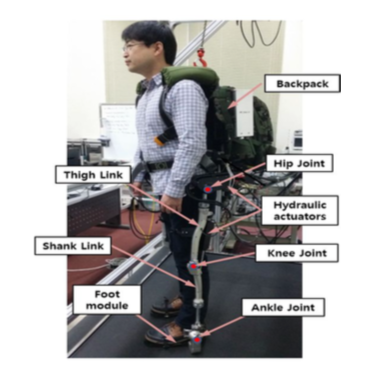
\includegraphics[width=3.in]{exos/figs/hydLowerExrem/exoSuit}
  \caption{Exoskeleton robot system.}
%  \vspace{-0.2in}
 \label{fig:exoSuit}   
 \end{figure} 
 

\subsection{Actuator specifications}

The Hydraulic Lower Extremity Exoskeleton's actuators were designed based on human walking data obtained at 4km/h with a 45 kg load.  Based on this data, the hydraulic capacity system was designed to provide 2050psi and 8lpm.  The individual actuators were designed to be double acting at the hip and knee flexion/extension joints. They provide a {\bf hip maximum thrust of 4 kN} and {\bf knee maximum thrust of 4 kN}.  Each joint joint includes three-way servo valves (M 200, Star-Hydraulic) to control rate and direction of bi-directionality, and bypass valves to connect the pump path to tank path for fast, energy-efficient motion during swing phases.   

The hydraulic system for each joint is shown in Figure \ref{fig:hydraulicSys}.
A picture of the Hydraulic Lower Extremity Exoskeleton is presented in Figure \ref{fig:exoSuit}.
\begin{figure}[thpb]
\centering
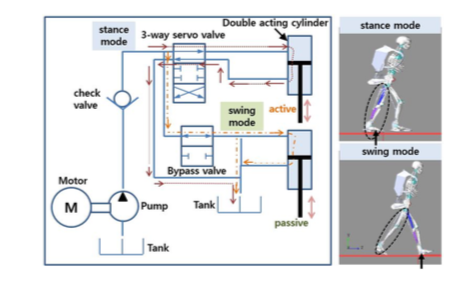
\includegraphics[width=3.in]{exos/figs/hydLowerExrem/hydraulicSys}
  \caption{Dual-mode control}
%  \vspace{-0.2in}
 \label{fig:hydraulicSys}   
 \end{figure} 


%\begin{figure}[thpb]
%\centering
%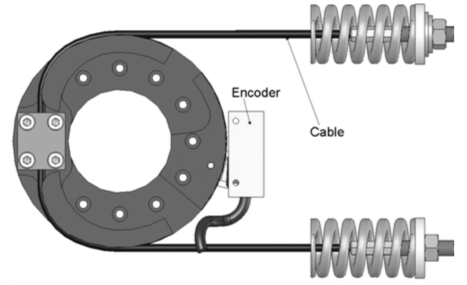
\includegraphics[width=3.in]{figs/seaAssm}
%  \caption{}
%  \vspace{-0.2in}
% \label{fig:IHMCSEA}   
% \end{figure}
 

 
 \subsection{Exoskeleton Specifications}
 
 The Hydraulic Lower Extremity Exoskeleton includes four actively controlled joints in the sagittal plane, with powered knee and hip flexion/extension.  The eight passive joints include one ab/adduction DOF for each hip and 3 DOF for each ankle.
 
 The hydraulic system is composed of the four actuators and a hydraulic power unit, consisting of a pump, motor, temperature sensor, and various valves.
 
 On-board sensors measure \textbf{joint angles}, \textbf{actuator forces}, and \textbf{ground reaction forces}.  Three \textbf{absolute angular encoders} are incorporated at the hip, knee, and ankle pitch joints.  In-line \textbf{load cells} are incorporated in each cylinder tube to measure actuator forces, and four single axis load cells are included in foot sensors to be used for gait phase detection.
 
 \subsection{Control Specifications}
 
 \begin{figure}[thpb]
\centering
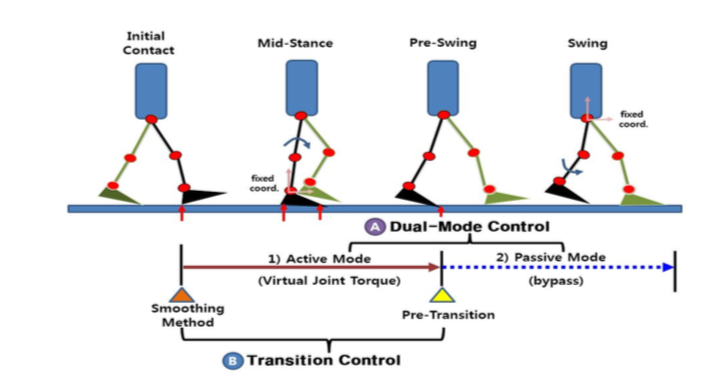
\includegraphics[width=5.in]{exos/figs/hydLowerExrem/dualModeDia}
  \caption{Locomotion control strategy during gait : Smoothing method ! Active mode ! Pre-transition method ! Passive mode}
%  \vspace{-0.2in}
 \label{fig:dualModeDia}   
 \end{figure}
The control design principle for the Hydraulic Lower Extremity Exoskeleton is based on the concept that, for walking gaits, the {\bf stance and swing controllers should be considered separately}.  To this end, the control designers developed an active-passive control method called {\bf Dual-Mode Control}.  Active control is used during stance phases whereas the passive control is used to quickly and freely control the system's legs during swing phases.  Additionally, to handle the inherently discontinuous jumps in the command signals that occur in this dual mode abstraction, a smoothing method is used in conjunction with a pre-transition method that solves for the swing delay due to internal cylinder pressure.  A diagram which highlights the different modes in this control strategy is in Figure \ref{fig:dualModeDia}.   

Various components of the dual-mode control strategy, at the hardware level, are presented in Figure \ref{fig:suitDia}.  
  \begin{figure}[thpb]
\centering
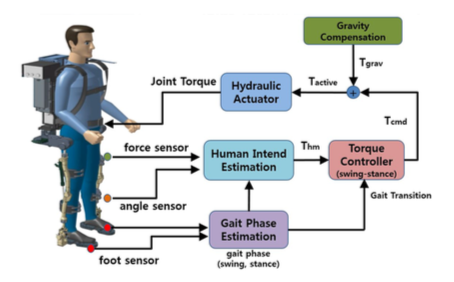
\includegraphics[width=3.in]{exos/figs/hydLowerExrem/suitDia}
  \caption{Overall control block diagram.}
%  \vspace{-0.2in}
 \label{fig:suitDia}   
 \end{figure}
This figure contains a {\bf gait phase estimation block}, which uses the foot sensors to estimate the stance mode of the system, a {\bf human intention block}, which uses angular encoders and joint force sensors to estimate the motion of the operator, a {\bf torque controller}, and a {\bf gravity compensation} block.  Note that these various components of the control system are used to support the general assumption of the dual mode controller, i.e., 
 \begin{figure}[thpb]
\centering
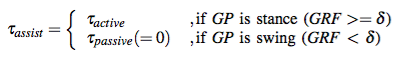
\includegraphics[width=3.in]{exos/figs/hydLowerExrem/torAssist}
%  \caption{Simplified virtual joint torque control block diagram}
%  \vspace{-0.2in}
% \label{fig:suitDia}   
 \end{figure}
 %
 \noindent
where, $GP$ is the gait phase, $GRF$ is the ground reaction force, and $\delta$ is a threshold value.  This equation explicitly states that an active torque will be applied for each leg during stance and that the legs are passive in their respective swing phases.

Like other controllers presented in this report, the dual mode control method in this section uses the fundamental assumption that it is difficult to measure the interaction forces between the user and hardware system directly as a primary design principle.  To this end, the human-robot interaction force is assumed to be completely represented in terms of the joint torque applied by the operator in the hardware. 

To calculate the active torque applied to the joints during the active mode control, the robot dynamics are considered independently from the operator, namely,
\begin{equation}
\vT_a = \mM(\vq)\ddot{\vq} + \mC(\vq,\dot{\vq})\dot{\vq}+\mG(\vq),
\label{dynamics}
\end{equation}   
where $\vT_a$ is the joint torque applied by the actuators, $\mM(\vq)$ is the inertia matrix, $\mC(\vq,\dot{\vq})$ is the centripetal and Coriolis matrix, and $\mG(\vq)$ is the gravitational torques. note that this equation neglects friction as well as other actuation dynamics.

Using the force sensors on the hydraulic actuators, the {\bf human-robot interaction torques} can be approximated as
\begin{equation}
\hat{\vT}_{hm} = \mM_n(\vq)\ddot{\vq} + \mC_n(\vq,\dot{\vq})\dot{\vq} + \mG_n(\vq) - \hat{\vT}_a, \notag
\end{equation}
where $\mM_n$, $\mC_n$, and $\mG_n$ are the nominal models of the true inertia, centripetal, and gravitational parameters and $\hat{\vT}_a$ represents the measured actuator torques.  The $\mM_n(\vq)\ddot{\vq} + \mC_n(\vq,\dot{\vq})\dot{\vq} + \mG_n(\vq) $ portion of $\hat{\vT}_{hr}$ represents the inverse dynamics component of the closed-loop control system.  The overall joint torque controller, which combines compensation for operator intent as well as balancing of the suit under a gravitational load, is then written \[ {\bf\tau}_\text{active} = K(s) \hat{\vT}_{hm} + \mG_n(\vq),\] where $K(s) = K_p +s K_d,$ i.e., there is closed-loop PD control law operating on the error between the predicted robot dynamics and the measured joint torques.  The block diagram for the active mode controller is shown in Figure \ref{fig:blockDia}. 
 \begin{figure}[thpb]
\centering
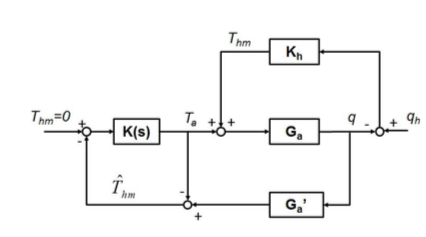
\includegraphics[width=3.in]{exos/figs/hydLowerExrem/blockDia}
  \caption{Simplified virtual joint torque control block diagram.}
%  \vspace{-0.2in}
 \label{fig:blockDia}   
 \end{figure}
 Note that $\mG_a$ represents the dynamics of the the system and $\mG_a'$ the inverse dynamics model in Figure \ref{fig:blockDia}.

 In the passive mode, which occurs during the swing phase, the leg of the human-robot system moves quickly and freely under using the passive inertial forces of the overall system.  This is accomplished using bypass valves that connect the pump and tank paths to achieve mechanical back-drivability.  The foot sensors trigger the bypass valves and to initiate the pass control mode.

The Hydraulic Lower Extremity Exoskeleton uses a novel scheme to manage transitions between the active and passive control modes.  In particular, the controller applies an explicit smoothing method to address discontinuities in the command torque at phase transitions.  The implementation proposed uses an exponential weighting function of the form
 \begin{figure}[thpb]
\centering
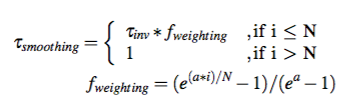
\includegraphics[width=3.in]{exos/figs/hydLowerExrem/weightingForm}
%  \caption{Simplified virtual joint torque control block diagram.}
%  \vspace{-0.2in}
% \label{fig:suitDia}   
 \end{figure}
 
 \noindent
 where ${\bf\tau}_\text{inv}$ is the inverse dynamics torque associated with the robot model, $f_\text{weighting}$ is the weighting function, $a$ is a sensitivity factor, and $N$ describes the duration of the transition period.  The transition duration period as well as sensitivity factor appear to be hand tuned parameters. 

In addition to phase transition smoothing, a pre-transition control method is applied at the end of the stance phase prior to the passive swing phase in order to affect smooth phase transitioning.  The pre-transition control works by measuring the ground reaction force and setting a minimum threshold value.  When the GRF drops below the threshold the system enters a passive swing control mode, i.e., the bypass valve at the actuators are opened.  The objective of this method is to reduce the phase transition delay due to residual pressure in the foot sensors. 


 
 \subsection{Assessment and Recommendations}
 
The design of the Hydraulic Lower Extremity Exoskeleton has a lot going for it.  The best part of this hardware as well as control design is the fact that the creators of it are doing something relatively straightforward.  The actuators are composed of what appears to be off-the-shelf components, and the addition of bypass valves to take advantage of passive dynamics during walking to produce more energy conscious behaviors is a good idea.    

One potential drawback of this hardware is the power system.  The documentation in \cite{} was sparse with respect to the exact specifications of the motor and energy storage device which powers the hydraulic system.

The control system for this hardware followed a relatively straight-forward design, effectively creating a ``get out of the way design" using the torque sensed at the joints only.  In the short-term, this type of policy seems to be a good strategy.  The other highlight of the outlined control policy was the smoothing function which was used during phase transitions in the walking gait cycle.  A similar type of smoothing will most likely be beneficial in terms of operator experience for a varity of different operational modes in which different phase transitions occur, e.g., running, jumping, etc.
 
The figures as well as hardware and control specifications in this section are taken from \cite{dual_mode_2015}.
 
\printbibliography[heading=subbibliography]

\end{refsection}

 
 % \end{document}

 
 % Hongchul Kim and Changhoon Seo and Young June Shin and Jung Kim and Youn Sik Kang, "Locomotion Control Strategy of Hydraulic Lower Extremity Exoskeleton Robot," IEEE International Conference on Advanced Intelligent Mechatronics, 2015, pp. 577-582.
 
 
 

%%% Local Variables:
%%% mode: latex
%%% TeX-master: "../survey"
%%% End:
